\documentclass[final,a4j,12pt]{jreport}
\newfont {\boldmathl}{cmmib10 scaled\magstep1}
\newcommand{\bm}[1]{\mbox{\boldmathl #1}}
\newcommand{\lw}[1]{\smash{\lower2.0ex\hbox{#1}}}

\usepackage{multicol}
\usepackage{amsmath,amssymb}

\usepackage[dvipdfmx]{graphicx}
\usepackage{textcomp}
\usepackage{plext}
\usepackage{enumerate}
\usepackage{epsfig}
\usepackage{comment}
\usepackage{longtable}
\usepackage{here}
\usepackage{./stylefile/cite}
\usepackage{./stylefile/jverb}
\usepackage{./stylefile/here}
\usepackage{./stylefile/bpaper}
\usepackage{./stylefile/epsbox}
\usepackage{./stylefile/fancyheadings}
\usepackage{./stylefile/slashbox}
\usepackage{./stylefile/subfigure}
\bibliographystyle{jplain}

\def\frac#1#2{\genfrac{}{}{}{}{\;#1\;}{\;#2\;}}
\def\dfrac#1#2{\genfrac{}{}{}{0}{\;#1\;}{\;#2\;}}
\def\tfrac#1#2{\genfrac{}{}{}{1}{\;#1\;}{\;#2\;}}
\def\sfrac#1#2{\genfrac{}{}{}{2}{\;#1\;}{\;#2\;}}
\def\ssfrac#1#2{\genfrac{}{}{}{3}{\;#1\;}{\;#2\;}}

\usepackage{tabularx}
\newcolumntype{Y}{>{\centering\arraybackslash}X}
\newcolumntype{Z}{>{\raggedleft\arraybackslash}X}

\usepackage{url}
\renewcommand{\url}{\begingroup \def\UrlLeft{}\def\UrlRight{}\urlstyle{rm}\Url}

\def\so{.\raisebox{1ex}{.}.\quad}
\def\because{\raisebox{1ex}{.}.\raisebox{1ex}{.}\quad}
\def\Omicron{O}
\def\omicron{o}

\newcommand{\pdif}[2]{\frac{\partial #1}{\partial #2}}

\setcounter{secnumdepth}{6}
\makeatletter
\newcommand{\subsubsubsection}{\@startsection{paragraph}{4}{\z@}
  {1.5\Cvs \@plus.5\Cdp \@minus.2\Cdp}
  {.5\Cvs \@plus.3\Cdp}
  {\reset@font\normalsize\sffamily}
}

\def\bs#1{\boldsymbol{#1}}
\def\quot#1{``#1''}
\def\ggn{Google {\it N}-gram}


\addtolength{\topmargin}{-15mm}
\addtolength{\oddsidemargin}{-15mm}

\newcommand{\argmax}{\mathop{\rm argmax}\limits}
\newcommand{\argmin}{\mathop{\rm argmin}\limits}

\begin{document}
\begin{titlepage}
\thesis
{負の報酬を考慮したIL-RBMの強化学習タスクへの応用}
{Application of IL-RBM Considering Penalty to Enforcement Learning}
{萩原 将文 教授}
{今井 倫太 教授}
{27}
{学籍番号 61214423}
{中村 晃貴}
\end{titlepage}
\pagenumbering{roan} 
\contents
\pagenumbering{arabic}


\abstract
fffffffffffffffffffffffffffffffffffffffffffffこ
%%!TEX root = ../main.tex
\chapter{はじめに}

近年、機械学習についての研究が盛んである。機械学習の学習手法は大きく三つに分類され、それぞれ教師あり学習、教師なし学習、強化学習である。とりわけ、強化学習は複雑で正確な教師データの与えられない実環境において、ロボット制御や最適化をおこなう有望な手法として注目されている。また、近年のディープラーニング (深層学習: Deep Learning) の成功をうけ、ディープニューラルネットワークを用いた強化学習に対する研究も盛んに行われている。そのような研究の中でも最も有名な研究の一つとして、ディープラーニングと強化学習を組み合わせビデオゲームを解いたものがある[Mnih 13]。この研究では、ディープニューラルネットワークを用いて行動価値観数を近似する手法を用い、複数種のビデオゲームにおいて人間を上回る性能を学習させることに成功した。

一方ニューラルネットワークの学習手法に対する研究も盛んに行われている。一般にニューラルネットワークの学習には多くのパラメータを設定する必要がある。また、ニューラルネットワークは、新規のデータを学習させた場合、過去に学習したデータを忘却する、破壊的干渉と呼ばれる現象がおこる [津守 10]。

これらの問題点を解決するため、多くの手法が提案されてきた。ニューラルネットワークの学習におけるパラメータは、学習率、素子数、層数など多く存在する。例えば、学習率の自動決定として、Adagrad[Duchi 11], やAdam[Kingma, 15]といったものが提案されている。

また、素子数についての研究としてBengioらによる研究[]などがある。この研究ではRBMの中間素子数がデータ数+1であれば理論上データセットを完全に学習できることが示された。しかしながら実際に使用される際のRBMの主要な役割はデータセット内から特徴を抽出することであり、この役割においてデータセットを完全に学習してしまうような素子数を設定することは適切ではない。

ニューラルネットワークは追加学習が出来ないという点について、大澤らは素子を新たに追加するRBMを提案することで、既学習情報を破壊せず追加学習を可能にした[大澤 14]。RBMに対し与えられた学習データを未学習か既学習かを判定し、未学習であれば新たに素子を追加し学習を行うことで、追加学習を行った。

また、大澤は彼らの提案したRBMを強化学習、行動選択タスクに対し応用した。提案したRBMに正の報酬が与えられた際の環境と行動を学習させた。その後、与えられたデータを未学習が既学習かを判定するプロセスを応用することで、新たに選択する行動によってもたらされる環境が、学習済みの環境か否かを判別し、最適行動選択を行った。

しかし、大澤の提案したRBMではデータセットの未学習、既学習は判定できるものの、与えられたデータが正の報酬に関連づいたデータであるのか、負の報酬に関連ついたデータであるのかを判定することが出来ない。

本研究では大澤の提案したRBMを改良し、与えられたデータが正の報酬に関連したデータであるか、府の報酬に関連したデータであるかを判別可能なRBMを提案する。異なるデータセットに対しそれぞれネットワークを割り当てることで、異なる種類のデータに対して未学習、既学習を判定することが可能である。また、正の報酬に関連したデータセットを学習するネットワークと負の報酬に関連したデータセットを学習するネットワークを持つRBMを使用したエージェントを用い、簡単な強化学習タスクへと応用する。正の報酬が与えられた際の環境と行動、負の報酬が与えられた際の環境と行動をエージェントに学習させ、未学習、既学習を判定することで、長期的な観点から正の報酬を獲得し、負の報酬を避けようとする最適行動選択が可能であることを示す。

以下、2章で既存手法の説明をし、3章で提案手法について詳細を述べ、4章で評価実験について示し、5章をまとめとする.


%%!TEX root = ../main.tex
\chapter{Restricted Boltzmann Machineの特徴と欠点}
この章では、本研究で改良を加えるRestricted Boltzmann Machineniについて具体的に述べる。

\section{ニューラルネットワーク}
ニューラルネットワークは、神経科学的な特徴を反映させた計算モデルである。人間の脳のニューロンとシナプスを模しており、ある値を持つノード(人口ニューロン)とその結合荷重によって表現される。

近年、多層に重ねたニューラルネットワークを用いたディープラーニングが画像認識や音声認識などのパターン認識や、データマイニングにおいて非常に目覚ましい成果を上げており、近年注目を集めている。

\section{ニューラルネットワークの問題}
ニューラルネットワークは、多次元量の線形分離不可能なデータを比較的少ない計算量で扱えるといった長所がある一方、以下に列挙するような問題をはらんでいる。

\subsection{破壊的干渉}
あるデータセットを学習済みのニューラルネットワークに対し、新たなデータセットを学習させる際、既に学習したデータを忘却してしまう、という問題がある。これを破壊的干渉という。

異なる性質のデータセットをその違いを考慮し、一つのニューラルネットワークで扱う場合、既学習情報を破壊せず新たなデータセットを学習する必要がある。

このような問題を解決するために、学習データを保持し、新たなデータセットと合わせて学習するという手法が提案された。しかし、このような手法は学習データを保持し続けなければならず、学習時間が長くなり、メモリを大量に必要とする、という欠点がある。

\subsection{メタパラメータの設定}
ニューラルネットワークの学習には、様々なメタパラメータの設定が必要不可欠である。例えば、層の数、それぞれの層におけるノード数、学習率、荷重減衰、モーメンタムなどである。このようなメタパラメータの組み合わせは莫大な数に上り、これらのパラメータの異なるそれぞれのモデルに対し、それぞれ学習を行い予測精度を比較することは、手間と時間が非常にかかる。そのため、これらのメタパラメータの自動決定、最適化は非常に需要のある研究である。

データセットに対し、データセットの特徴を十分学習する素子数の計算する研究がある。

また、学習率の自動決定に関しては、多くの手法が提案されており、その例として、Adagrat、Adamなどが挙げられる。

\subsection{局所解への収束問題}
ニューラルネットワーク、特に多層ニューラルネットワークにおいて、局所解への収束問題は非常に重要な問題である。ニューラルネットワークの学習において基本的に用いられる手法に誤差逆伝播法があるか、この誤差逆伝播法は設定された誤差関数を現象させるようにノード間の結合荷重などのパラメータを調整する。したがって、誤差関数の局所解へ収束していしまい、最適解へ辿りつけないという問題がある。

局所解への収束問題はとりわけ多層ニューラルネットワークにおいて顕著であり、局所解への収束問題を解決するために事前学習(pre-training)という手法が提案されている。


\section{Restricted Boltzmann Machine}
Restricted Boltzmann Machine(RBM)とは、ニューラルネットワークの一種である。

統計的な変動を用いたホップフィールドネットワークの一種であるBoltzmann Machineの、可視層間、隠れ層間の結合を制限したものである。

その学習における結合の重みの変化の過程が、脳における神経科学的な学習則であるヘブ則とも類似しているなど、ニューラルネットワークの現在非常に有力な手法の一つである。

RBMは可視層と隠れ層の二層からなる。可視層に入力データを入れ学習させることで、隠れ層にその特徴をよく表すようなパラメータが出力される、という特徴がある。

通常、可視層、隠れ層の各ノードには0か1の値が入る。可視層に入力データを入れることで、隠れ層の各ノードの取る値の条件付き確率が計算できる。ゆえに、RBMは確率モデルであり生成モデルである。

\section{Deep Belief Network}
Deep Belief Network(DBN)とは、Deep Neural Networkの一種である。

Deep Neural Networkの一般的な学習方法である、誤差逆伝播法の問題の一つに、局所解への収束問題がある。
誤差逆伝播法はある誤差関数を最小化するように各パラメータを変化させる手法であるが、その性質上誤差関数の局所的な解に収束し、誤差関数の最適解へ収束しない現象が起こり得る。
この現象はDeep Neural Networkの層数が増えるに従ってより起こりやすくなる。
この局所解への収束問題を解決する手法として事前学習(pre-training)が考案された。

事前学習の手法にはいくつかあるが、そのうちの一つが前述したRBMを用いるもので、RBMを用いた事前学習を行うDeep Neural NetworkをDBNと呼ぶ。

DBNではRBMを多段に重ねた構造を取る。
そして、一番下の層から入力データをRBMに学習させ、RBMの隠れ層に特徴が現れるよう各パラメータを学習させる。
その後、RBMが生成モデルである利点を活かし、一番下の層に入力データを入れた後に計算される、隠れ層の条件付き確率を次層のRBMにの可視層に入力し、同じように特徴を学習させる。

このようにしてパラメータを学習させたDeep Neural Networkは、それぞれの層において入力データの特徴をうまく抽出するようパラメータが決定されているため、初期パラメータをランダムに決めていた多層パーセプトロンに比べ局所解へ収束しづらい。

こうして事前学習されたネットワークを最後に教師あり学習で学習させる(fine-tuning)手法をDBNと呼ぶ。

\section{強化学習}

%%!TEX root = ../main.tex
\chapter{システムの概要}
この章ではシステムの概要について説明する。


\section{システム全体の構成}
本システムは、強化学習の基本的な考え方に則り、"環境"と"エージェント"が”行動"と"報酬"により相互に影響を及ぼし合うように構成されている。

\subsection{システム全体の流れ}
システムの流れは以下のとおりである。

\begin{enumerate}
  \item 二つのエージェントを定義する。
  \item 先行のエージェントに盤面の状態を与える。
  \item 先行のエージェントは盤面の状態から行動を選択する。
  \item 環境は、エージェントの行動を受け取り、自身の状態を更新する。
  \item 環境の状態に応じて、エージェントに報酬を与える。
  \item 環境の状態が終了条件を満たせばゲームを終了する。
  \item 上記手順を先攻、後攻を交代し繰り返す。
\end{enumerate}



環境部分は、常にある状態をを持ち、その状態はエージェントの行動によって変化させられる。また、環境部はその状態とエージェントの行動によってエージェントに与える報酬を決定する。

\section{Incremental Learning-RBM(IL-RBM)}

この節では、本システムの根幹となるIL-RBMについて説明する。
IL-RBMは追加学習を行うと既学習情報を失うというRBMの欠点を改良したものである。

\subsection{追加学習}
IL-RBMでは追加学習を行う。追加学習とは、既にあるデータセットに対し学習済みのニューラルネットワークが、新たなデータセットに対し、既学習情報を失わない形で学習を行うことである。

通常のRBMの隠れ層のノード数は一定である。しかし、IL-RBMは新たなデータセットを学習する際に隠れ層のノード数を追加する操作を行う。IL-RBMの学習は次のような流れをとる。

\begin{enumerate}
  \item 初期データセットに対しIL-RBMを学習させる。
  \item 追加データセットに対し、適切な追加ノード数を決定し、Il-RBMの隠れ層にノードを追加する。
  \item 上記手順で追加したノードのみを用いて、追加データセットを学習させる。
  \item 上記2、3の手順を追加データセットの分だけ繰り返し行う。
\end{enumerate}



\section{IL-RBMの強化学習への応用}
本システムでは、IL-RBMを用いて強化学習タスクを行う。IL-RBMを用いたエージェントを設定し、このエージェントに、ある環境下において得られる報酬を最大化するような行動を学習させる。

\subsection{強化学習}
強化学習とは、あるエージェントがある環境内にて、得られる報酬を最大化するような行動を学習するような機械学習のことである。

強化学習には重要な4つの概念がある。

\begin{itemize}
  \item 環境 … エージェントの行動に応じて、報酬をエージェントに与える。また、エージェントの行動に応じて、エージェントの観測する環境も更新される。
  \item 報酬 … エージェントの行動に応じて環境からエージェントに与えられる。この得られる報酬を最大化するようエージェントは行動を学習する。
  \item 行動  … エージェントは観測した環境に応じて、行動を選択する。
  \item エージェント … 環境を観測し、報酬を受け取り、行動を選択する。
\end{itemize}

明確な教師データが与えられる教師あり学習や、全く教師データが与えられない教師なし学習と異なり、報酬という限定されたフィードバックのみが与えられる点に特徴がある。
不確実な環境を取り扱えるという点で、応用上非常に有望な機械学習手法の一つである。


\subsection{未学習データセットの判別}
エージェントに与えられたあるデータを既学習であるか、未学習であるかを判別する手法について述べる。
エージェントに与えられたデータの既学習判定にRBMのエネルギーを用いる。RBMは学習済みのデータに対して、エネルギーが低くなる、という特徴を持つため、データを入力した際のRBMのエネルギーを見ることで入力されたデータが既学習であるか、未学習であるかを判別することができる。


\subsection{エージェントの概要}
エージェントの概要について具体的に説明する。

本システムで用いたエージェントは、IL-RBMと出力層からなるDBN(以下、IL-DBN)を用いている。このIL-DBNは入力データを環境、出力を行動として学習する。
エージェントは、常に今自分が置かれている環境を観測することが可能であり、環境から報酬を与えられた場合には、それを感知することが可能である。

エージェントは環境と行動の組からなるデータセットを自動的に構築し、そのデータセットを逐次的に学習することで、最適行動を学習する。
また、IL-RBMのエネルギーに注目することで、未学習データセットを検出できるという特徴を用い、後述するサブゴールを獲得し、長期的な戦略を獲得することが可能である。


\subsection{データセットの獲得}

本システムがデータセットを環境中から自動で学習するメカニズムについて説明する。
以下、三目並べタスクの最適行動を学習するエージェントを例に説明する。

学習エージェントが対戦相手と三目並べを行う環境下で、三目並べに勝利した場合と敗北した場合にそれぞれ正の報酬と負の報酬を与えられるとする。この時、エージェントが観測する環境は盤面の状態であり、出力する行動は次に選択する手の盤面上の位置となる。

\subsubsection{勝利データセットの獲得}
まず、エージェントは勝利データセットを収集する。ある行動を出力した際、盤面が勝利条件を満たし、正の報酬が与えられたとする。その勝利条件を満たした際の行動と、その行動をとった際の環境を組みにしてデータセットとしてエージェントは保存する。

データセットがある一定数に達した場合、または試行回数が一定数に達した場合、エージェントは保存したデータセットを用いて学習を行う。

\subsubsection{サブゴールの獲得}
前述した、既学習、未学習判定を用いてサブゴールを獲得し、長期的な戦略を獲得するメカニズムについて説明する。

勝利データセットの獲得において、盤面が勝利条件を満たした場合、その時にとった行動と、行動を選択した際の環境を組みにしてデータセットとして保存した。
この場合、勝利条件を満たした盤面の状態をゴールとしてデータセットを採集している。

サブゴールとは、ゴールにつながり得る環境の状態を指す。
サブゴールを適切に設定し、サブゴールに至る行動と、その行動を選択した際の環境を更にデータセットに加える事で、長期的な戦略を獲得することができる。

サブゴールの設定方法について説明する。ある行動を選択し、環境が更新されたとする。
その際の環境をエージェントのRBMが既学習であるか未学習であるかを前述したエネルギーによる判定法で判定する。
そして、得られた環境が既学習であった場合、その環境はゴールへと至る可能性が高いため、その環境をサブゴールとして設定する。
そして、サブゴールに至る直前の環境と、その状態にて選択した行動をデータセットとして新たに保存し、追加学習を行う。

このようにして、サブゴールについても学習したIL-RBMは、また新たに"サブゴールのサブゴール"を扱うことが可能になる。観測された環境が、既に学習済みであるサブゴールである環境と一致、近似すると判定された場合、さらにその環境に至る行動とその直前の環境をデータセットとして加えることで、サブゴールのサブゴールを学習でき、長期的な戦略を獲得することが可能である。

\subsection{負のネットワーク、負のサブゴール}
前述したサブゴールの設定法には負の報酬と行動の抑制を扱えない、という欠点があった。
あるRBMがある環境を表す入力データを未学習か既学習か判定できたとしても、その環境が正の報酬に紐付いているか、負の報酬に紐付いているかを判定できないからである。

そこで、負の報酬と負の報酬を得る環境へ至る行動を抑制するために負の報酬をあつかうネットワークをエージェントに追加することにした。

エージェントはIL-RBMを二つ使用する。それぞれ正の報酬を扱うネットワークと負の報酬を扱うネットワークである。
また、保持するデータセットも二種類用意する。正の報酬を得ることのできるゴールに至る行動と、その直前の環境の組、サブゴールに至る行動とその直前の環境の組をデータセットとして扱う正のデータセットと、負の報酬について同様に扱う負のデータセットである。

負のデータセットを扱う負のネットワークでは、負の報酬を得ることになるゴール、サブゴールに至る行動が出力され、その直前の環境が入力データとなる。したがって、観測された環境をこのネットワークに入力した際の出力された行動は抑制されるべき行動である。

本エージェントでは負のネットワークからの出力を正のネットワークからの出力から引くことで、負の報酬を得る環境へ至る行動を抑制している。しかし、正のネットワークと負のネットワークを同列に扱うべきか、荷重をかけどちらかを優先すべきかなどは研究途中である。



%%!TEX root = ../main.tex
\chapter{IL-RBMの強化学習への応用}\label{ch:ilrbm}
この章では,IL-RBMを本システムにおける強化学習への応用について説明する.


\section{強化学習}
強化学習\cite{RL木村}とは,あるエージェントがある環境内にて,得られる報酬を最大化するような行動を学習するような機械学習のことである.

図\ref{fig:el}に示すように,強化学習には重要な4つの概念があり,それらが相互作用を行う.

\begin{figure}[tb]
 \begin{center}
  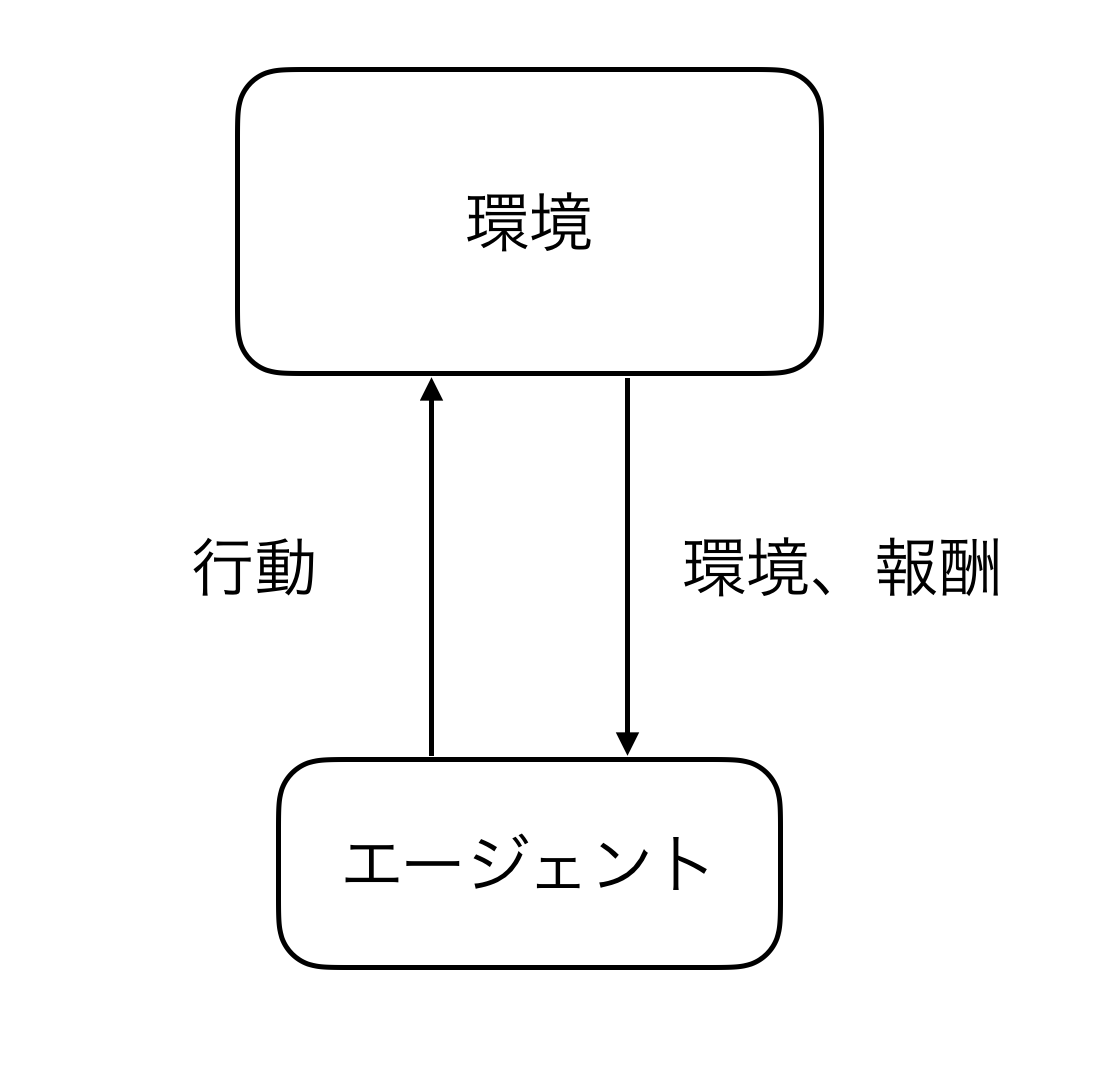
\includegraphics[scale=0.4]{./koki/el.png}
  \caption{強化学習の概要}
  % \ecaption{Representations of Data} 
  \label{fig:el}
 \end{center}
\end{figure}


\begin{itemize}
  \item 環境 … エージェントの行動に応じて,報酬をエージェントに与える.また,エージェントの行動に応じて,エージェントの観測する環境も更新される.
  \item 報酬 … エージェントの行動に応じて環境からエージェントに与えられる.この得られる報酬を最大化するようエージェントは行動を学習する.
  \item 行動  … エージェントは観測した環境に応じて,行動を選択する.
  \item エージェント … 環境を観測し,報酬を受け取り,行動を選択する.
\end{itemize}

明確な教師データが与えられる教師あり学習や,全く教師データが与えられない教師なし学習と異なり,報酬という限定されたフィードバックのみが与えられる点に特徴がある.
不確実な環境を取り扱えるという点で,応用上非常に有望な機械学習手法の一つである.

また,強化学習とニューラルネットワークを併用する研究も盛んであり,この分野で近年非常に有名になった研究に,ディープニューラルネットワークと強化学習の一手法であるQ学習\cite{watkins1992q}を組み合わせたDeep Q Networkと呼ばれる手法を提案し,それを用いてビデオゲームを解かせたものがある\cite{mnih2013playing}.

また,私達人間の脳内においても環境から与えられる報酬を予測していることが示唆されており\cite{schultz1997neural},上述した強化学習に近いメカニズムを脳内に持っていると予想されている\cite{銅谷}.
また,計算論神経科学の分野でも強化学習を人類の脳と関連付ける研究が盛んに行われている\cite{lee2012neural,izhikevich2007solving,maia2011reinforcement}.



\section{エージェントの概要}
エージェントの概要について具体的に説明する.

図\ref{fig:ildbn}に示す通り,本システムで用いたエージェントは,IL-RBMと出力層からなるDBN(以下,IL-DBN)を用いている.出力層はパーセプトロンで構成されている.このIL-DBNは入力データを環境,出力を行動として学習する.

\begin{figure}[tb]
 \begin{center}
  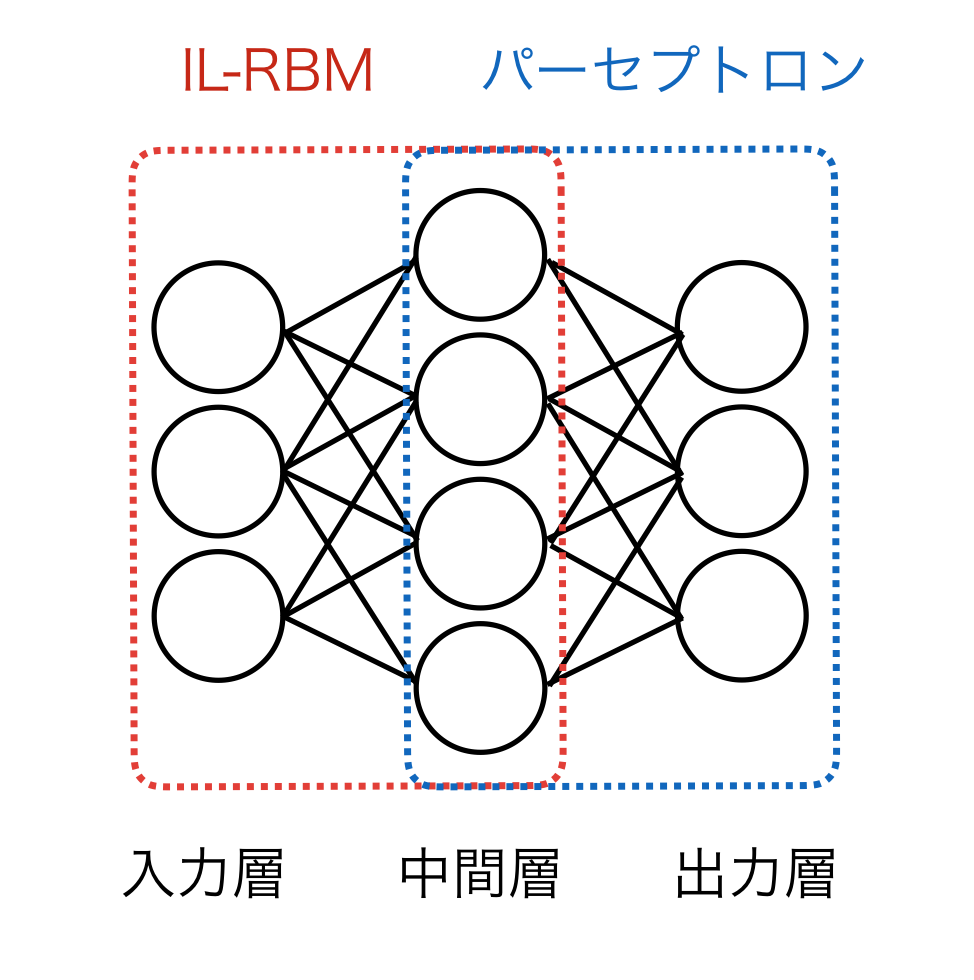
\includegraphics[scale=0.6]{./koki/ildbn.png}
  \caption{IL-DBN}
  % \ecaption{Representations of Data} 
  \label{fig:ildbn}
 \end{center}
\end{figure}


エージェントは,常に今自分が置かれている環境を観測することが可能であり,環境から報酬を与えられた場合には,それを感知することが可能である.

エージェントは環境と行動の組からなるデータセットを自動的に構築し,そのデータセットを逐次的に学習することで,最適行動を学習する.
また,IL-RBMのエネルギーに注目することで,未学習データセットを検出できるという特徴を用い,後述するサブゴールを獲得し,長期的な戦略を獲得することが可能である.どのようにデータセットを収集するかについての具体的手法について,次節から述べる.

\section{未学習データ判定法}

以下,文献\cite{osawa}内にて提案されている,未学習データ判別法について述べる.\ref{sec:learn}で説明したとおり,RBMは以下に$J$で表される対数尤度を最大化するように学習が行われる.すなわち,エネルギー$E$を最小化するように学習が行われることと同値である.

\begin{eqnarray}
	p(\bm{v}, \bm{h}; \theta) & = & \frac{1}{Z(\theta)}  \exp (-E(\bm{v},\bm{h};\theta)) \nonumber \\
	E(\bm{v}, \bm{h}; \theta) & = & -\sum_i b_i v_i - \sum_j c_j h_j- \sum_i \sum_j v_i W_{ij} h_j \nonumber \\
	p(\bm{v};\theta) & = & \sum_{\bm{h}} p(\bm{v},\bm{h};\theta) \nonumber \\
			& = & \sum_{\bm{h}} \frac{1}{Z(\theta)} \exp (-E(\bm{v}, \bm{h}; \theta)) \nonumber \\
	J & = & < \ln \sum_{\bm{h}} p(\bm{v}, \bm{h}; \theta) >_q \nonumber \\
	  & = & < \ln \sum_{\bm{h}} \exp (-E(\bm{v}, \bm{h}; \theta) >_q - \ln Z(\theta) \nonumber 
\end{eqnarray}

したがって,学習済みRBMは既学習データが入力された場合はエネルギーが低くなり,未学習データが入力された場合にはエネルギーが高くなる.この原理を応用し,あるデータが入力された際のRBMのエネルギーを判定することで未学習データか既学習データかの判定を行う.

未学習データを入力した際のエネルギーと既学習データを入力した際のエネルギーをそれぞれ記録しておき,この値に基づいてある閾値を決定し,未学習か既学習か不明であるデータが入力された際のRBMのエネルギーが,この閾値を上回れば未学習,下回れば既学習と判定する.

\section{データセットの獲得}

本システムがデータセットを環境中から自動で学習するメカニズムについて説明する.
以下,三目並べタスクの最適行動を学習するエージェントを例に説明する.

学習エージェントが対戦相手と三目並べを行う環境下で,三目並べに勝利した場合と敗北した場合にそれぞれ正の報酬と負の報酬を与えられるとする.この時,エージェントが観測する環境は盤面の状態であり,出力する行動は次に選択する手の盤面上の位置となる.

\subsection{勝利データセットの獲得}
まず,エージェントは勝利データセットを収集する.ある行動を出力した際,盤面が勝利条件を満たし,正の報酬が与えられたとする.その勝利条件を満たした際の行動と,その行動をとった際の環境を組みにしてデータセットとしてエージェントは保存する.

\begin{figure}[tb]
 \begin{center}
  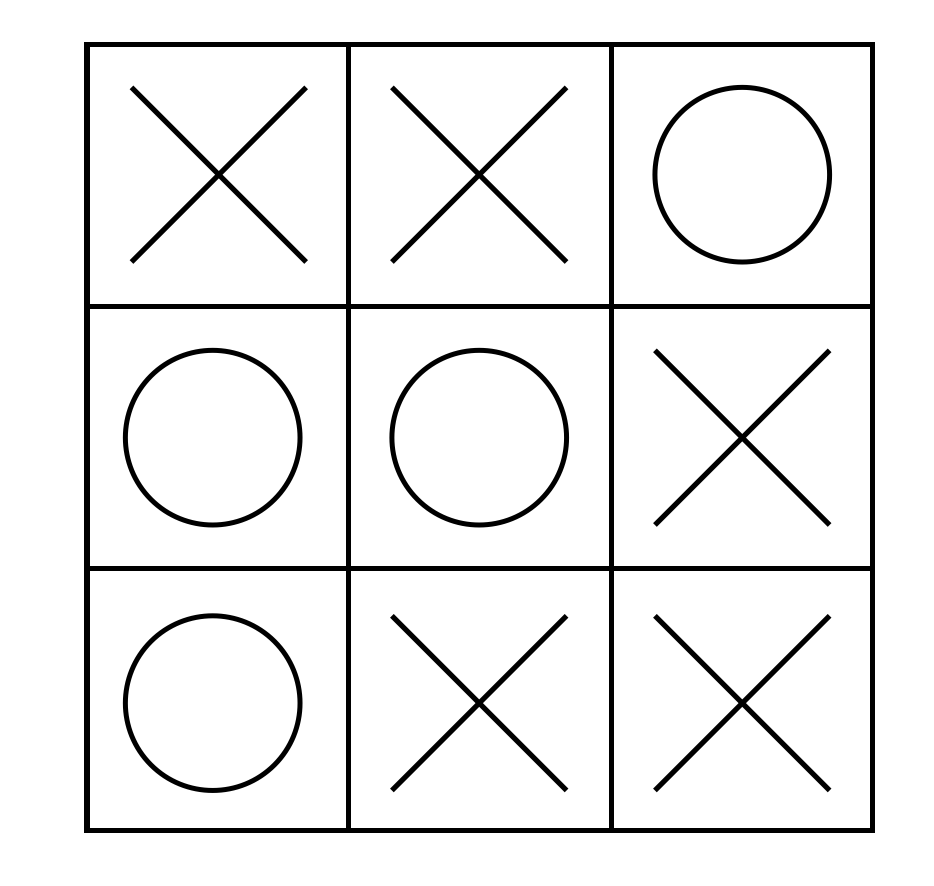
\includegraphics[scale=0.4]{./koki/ds.png}
 % ○が後攻,学習エージェント,
  %×が先行,相手エージェントを表す.
   \caption{勝利データセット例}
  % \ecaption{Representations of Data} 
  \label{fig:ds}
 \end{center}
\end{figure}

データセットがある一定数に達した場合,または試行回数が一定数に達した場合,エージェントは保存したデータセットを用いて学習を行う.

\subsection{サブゴールの獲得}
前述した,既学習,未学習判定を用いてサブゴールを獲得し,長期的な戦略を獲得するメカニズムについて説明する.

勝利データセットの獲得において,盤面が勝利条件を満たした場合,その時にとった行動と,行動を選択した際の環境を組みにしてデータセットとして保存した.
この場合,勝利条件を満たした盤面の状態をゴールとしてデータセットを採集している.

サブゴールとは,ゴールにつながり得る環境の状態を指す.
サブゴールを適切に設定し,サブゴールに至る行動と,その行動を選択した際の環境を更にデータセットに加える事で,長期的な戦略を獲得することができる.

\begin{figure}[tb]
 \begin{center}
  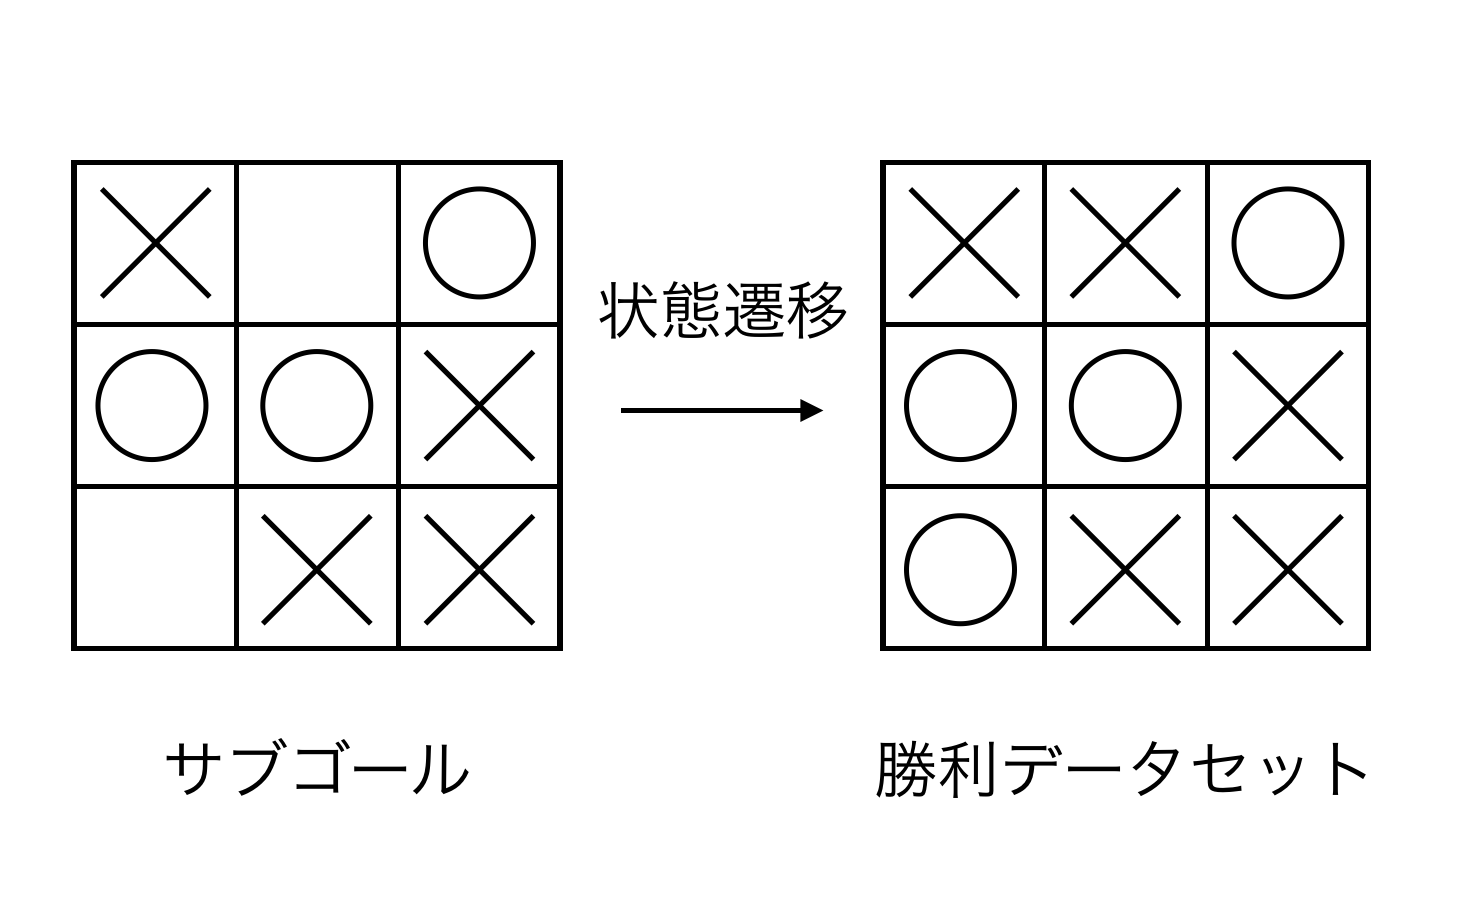
\includegraphics[scale=0.4]{./koki/sg.png}
   \caption{サブゴールの設定}
  % \ecaption{Representations of Data} 
  \label{fig:sg}
 \end{center}
\end{figure}


サブゴールの設定方法について説明する.ある行動を選択し,環境が更新されたとする.
その際の環境をエージェントのRBMが既学習であるか未学習であるかを前述したエネルギーによる判定法で判定する.
そして,得られた環境が既学習であった場合,その環境はゴールへと至る可能性が高いため,その環境をサブゴールとして設定する.
そして,サブゴールに至る直前の環境と,その状態にて選択した行動をデータセットとして新たに保存し,追加学習を行う.

\begin{figure}[tb]
 \begin{center}
  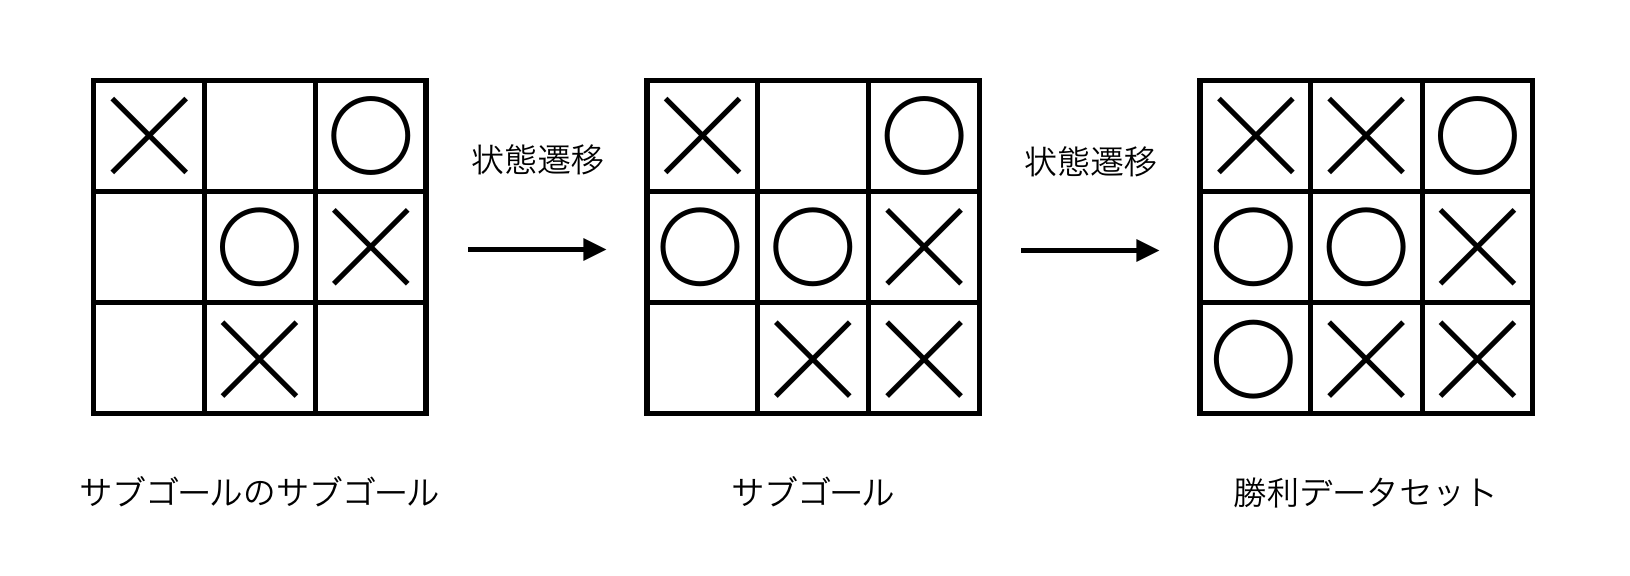
\includegraphics[scale=0.5]{./koki/sgsg.png}
   \caption{サブゴールのサブゴールの設定}
  % \ecaption{Representations of Data} 
  \label{fig:sgsg}
 \end{center}
\end{figure}


このようにして,図\ref{fig:sgsg}に示したとおり,サブゴールについても学習したIL-RBMは,また新たに'サブゴールのサブゴール'を扱うことが可能になる.観測された環境が,既に学習済みであるサブゴールである環境と一致,近似すると判定された場合,さらにその環境に至る行動とその直前の環境をデータセットとして加えることで,サブゴールのサブゴールを学習でき,長期的な戦略を獲得することが可能である.

\section{負のネットワーク,負のサブゴール}
前述したサブゴールの設定法には負の報酬と行動の抑制を扱えない,という欠点があった.
あるRBMがある環境を表す入力データを未学習か既学習か判定できたとしても,その環境が正の報酬に紐付いているか,負の報酬に紐付いているかを判定できないからである.

そこで,図\ref{fig:hn}に示すように負の報酬と負の報酬を得る環境へ至る行動を抑制するために負の報酬をあつかうネットワークをエージェントに追加することにした.

\begin{figure}[tb]
 \begin{center}
  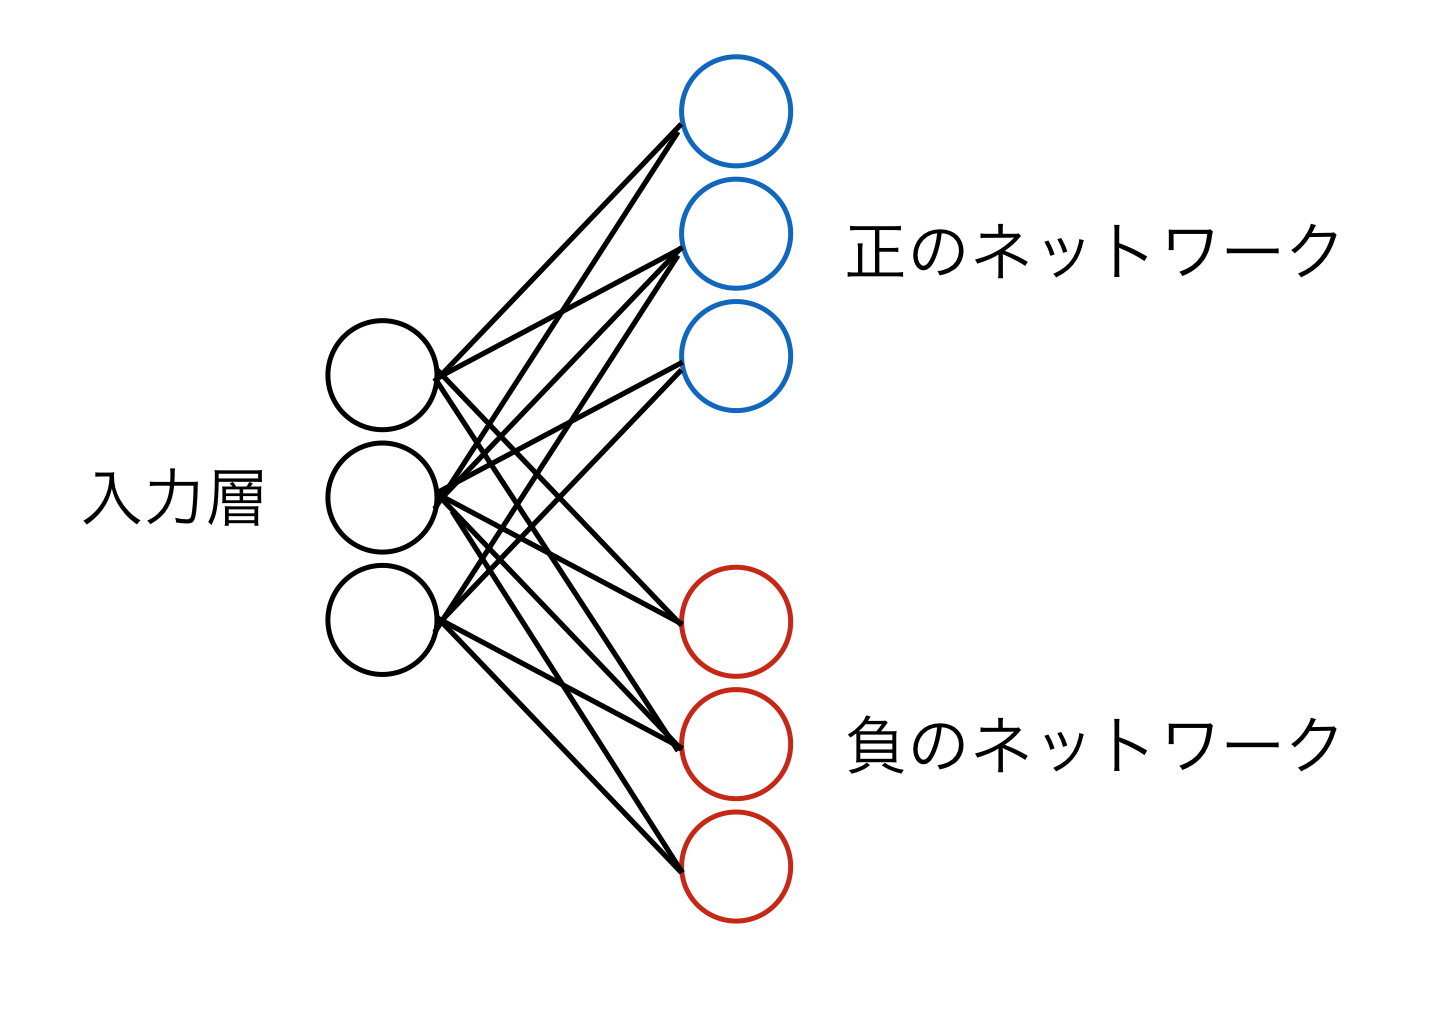
\includegraphics[scale=0.4]{./koki/hn.png}
  \caption{負のネットワーク}
  % \ecaption{Representations of Data} 
  \label{fig:hn}
 \end{center}
\end{figure}

エージェントはIL-RBMを二つ使用する.それぞれ正の報酬を扱うネットワークと負の報酬を扱うネットワークである.
また,保持するデータセットも二種類用意する.正の報酬を得ることのできるゴールに至る行動と,その直前の環境の組,サブゴールに至る行動とその直前の環境の組をデータセットとして扱う正のデータセットと,負の報酬について同様に扱う負のデータセットである.

負のデータセットを扱う負のネットワークでは,負の報酬を得ることになるゴール,サブゴールに至る行動が出力され,その直前の環境が入力データとなる.したがって,観測された環境をこのネットワークに入力した際の出力された行動は抑制されるべき行動である.

本エージェントでは負のネットワークからの出力を正のネットワークからの出力から引くことで,負の報酬を得る環境へ至る行動を抑制している.
%しかし,正のネットワークと負のネットワークを同列に扱うべきか,荷重をかけどちらかを優先すべきかなどは研究途中である.

\section{三目並べシステムの概要}

本システムは,強化学習の基本的な考え方に則り,'環境'と'エージェント'が'行動'と'報酬'により相互に影響を及ぼし合うように構成されている.

システムの流れは以下のとおりである.

\begin{enumerate}
  \item 二つのエージェントを定義する.
  \item 先行のエージェントに盤面の状態を与える.
  \item 先行のエージェントは盤面の状態から行動を選択する.
  \item 環境は,エージェントの行動を受け取り,自身の状態を更新する.
  \item 環境の状態に応じて,エージェントに報酬を与える.
  \item 環境の状態が終了条件を満たせばゲームを終了する.
  \item 上記手順を先攻,後攻を交代し繰り返す.
\end{enumerate}



環境部分は,常にある状態をを持ち,その状態はエージェントの行動によって変化させられる.また,環境部はその状態とエージェントの行動によってエージェントに与える報酬を決定する.

本システムは強化学習の基本的な考え方に則り,環境とエージェントの相互作用を取り扱う.

\subsection{環境部}
環境部はエージェントと環境の相互作用を制御するmainオブジェクトと,三目並べタスクの詳細の動作,情報を制御するThreePieceオブジェクトからなる.

\subsubsection{mainオブジェクト}
mainオブジェクトは,プログラム全体の制御を行う.

まず,行うタスクを定義する.今回行うタスクは三目並べであるためThreePieceオブジェクトをタスクとして定義する.その後,タスクの要請する数のエージェントを定義する.今回の実験では,先行のエージェントをランダムエージェント,後攻のエージェントをIL-DBNエージェントとした.

その他,エージェントと環境の相互作用を制御し,三目並べの終了時にThreePieceオブジェクトとエージェントのリセットを行ったり,三目並べを何ターン行うかの制御,それぞれのエージェント数の勝利数の保持を行う.

\subsubsection{ThreePieceオブジェクト}
ThreePieceオブジェクトは三目並べタスクを実際に執り行う.
ThreePieceオブジェクトはターン制でそれぞれのエージェントに盤面の情報を渡し,行動情報を受け取る.
盤面の情報の次元数や行動情報の形式はThreePieceオブジェクトが決定し,エージェントがアーキテクチャをその形式に合わせる.

盤面の情報はそれぞれのマスに対し,空白ならば(0,0),白石が置かれていれば(0,1),黒石が置かれていれば(1,0)の2bitで表現する.したがって9マス全体の表現は18次元の(0,0,0,1,1,0,0,0,0,1,0,0,0,0,0,0,1,0)のような表現になる.

一方エージェントの行動は0〜8の整数値で表される.それぞれの数値が石を置く盤面上の位置を示している.

%一方,エージェントの行動は9次元のベクトルで表現される.配置する石の位置に対応する次元の値のみ1で,それ以外は0のベクトルで表す.

ThreePieceオブジェクトはエージェントから渡された石の置き位置を示す値がルール上正当なものかを判定する.エージェントが石を置こうとしている場所に既に石が置かれている場合はエージェントに再度行動を選択するように命令する.指定された石の置き位置が正当であれば,オブジェクトの保持する盤面の状態を更新する.

その後,盤面の状態が三目並べの終了条件を満たしているかを判定する.盤面の状態を監視し,縦,横,斜めいずれかの方向に石が3つ並んでいれば,勝利エージェントへ報酬1を,敗北エージェントへ報酬-1を与える.

\subsection{エージェント部}
エージェントは基本的なエージェントの振る舞いを規定するAgentクラスがあり,それを継承することでそれぞれのAgentのクラスが作られている.

エージェントは環境から盤面状態を受け取った後,行動選択を行う.ランダムエージェントであれば0〜8で乱数を返し,学習エージェントは学習した行動を出力する.

環境が行動を受け取った後,エージェントは環境から報酬を受け取る.学習エージェントは報酬に応じて学習を行う.その学習の具体的なプロセスについては後述する.

\subsubsection{学習エージェント}
学習エージェントは次のような流れで学習を行う.


\begin{enumerate}
  \item 環境から状態が与えられる.
  \item 環境が記憶済みの状態の場合,一つ手前の状態とその状態でとった行動をデータセットに追加する.
  \item 行動選択後,環境から報酬が与えられる.
  \item 報酬に応じて状態と行動の組をデータセットに追加する.
  \item 上記の1から4を一定回数繰り返す.
  \item 採集したデータセット用いて追加するRBMのノード数を決定する.
  \item ノード数の確定したRBMを採集したデータセットで学習させる.
  \item データセットを空にリセットし1から再度データセットを採集する.
\end{enumerate}

学習エージェントには,負のネットワークを実装したものとしていないものの二種類あり,それらの勝率,敗北率を実験にて比較する.



%%!TEX root = ../main.tex

\chapter{評価実験}

\section{予備実験と各種パラメータの決定}\label{sec:lr}

学習率,エポック数等の各種パラメータを決定するために予備実験を行った.

\subsection{RBMの学習率とエポック数}
RBMの学習時の学習率は文献\cite{Hinton-guide}を参考に,更新量が重みの$10^{-3}$程度になるよう決定した.
学習エージェントが実際に採集した,入力を盤面の状態とし,出力を次に石を置く盤面の位置とするデータセットを利用する.RBMの素子数は\ref{sec:node}の自動決定法により決定した.


エポック数とクロスエントロピーの関係を以下の図\ref{fig:ep}に示す.

\begin{figure}[]
\begin{center}
   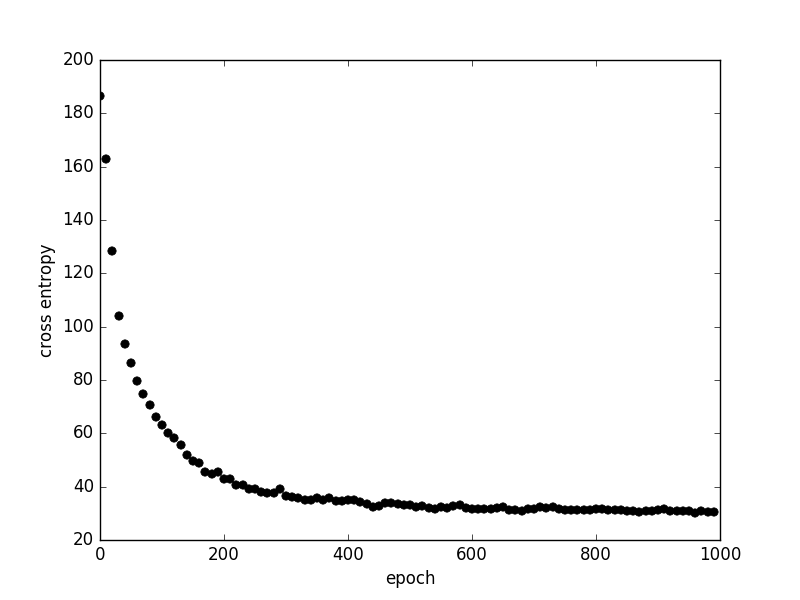
\includegraphics[scale=0.8]{./koki/l.png} \\
   \caption{RBM学習時のエポック数とクロスエントロピーの関係}
\label{fig:ep}
\end{center}
\end{figure}

以上の結果より,クロスエントロピーが確実に収束するエポック数としてエポック数を1000と決定した.

\subsection{出力層の学習率とエポック数}
出力層の学習率とエポック数を決定するため予備実験を行った.文献\cite{Hinton-guide}を参考に更新量が重みの$10^{-3}$程度になるよう決定した.
学習エージェントが実際に採集した,入力を盤面の状態とし,出力を次に石を置く盤面の位置とするデータセットを利用する.
RBMの素子数は\ref{sec:node}で説明した自動決定法により決定した.
エポック数と教師データと出力データの二乗和誤差との関係を以下の図\ref{fig:tu}に示す.

\begin{figure}[]
\begin{center}
   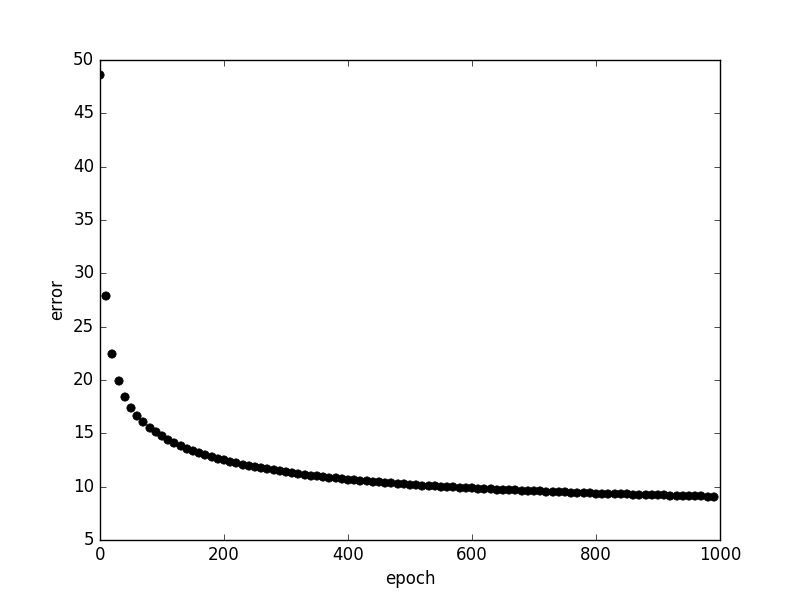
\includegraphics[scale=0.8]{./koki/t.png} \\
   \caption{RBM学習時のエポック数とクロスエントロピーの関係}
\label{fig:tu}
\end{center}
\end{figure}

以上の結果より,二乗和誤差が確実に収束するエポック数としてエポック数を1000と決定した.

\section{提案手法の評価実験}
予備実験にて決定した各種パラメータを用いて,評価実験を行った.

先行に対戦相手のランダムエージェント,後攻に学習エージェントを設定し,三目並べタスクを行った.

三目並べシステム,エージェントの詳細は\ref{ch:ilrbm}にて記述したとおりである.詳細な実験条件を\ref{tbl:exp}に示す.

エージェントは提案手法である負のネットワーク,負のサブゴールを実装したものと,既存手法の負のネットワークを実装していない既存手法\cite{osawa}の二種類を比較した.それぞれのエージェントに対し,勝率,敗北率,引き分け率を調査した.

各ターンごとの勝利数,敗北数,引き分け数を表\ref{tbl:r1},表\ref{tbl:r2}に示す.

\begin{table}[]
\begin{center}
	\caption{実験条件}
	% \ecaption{Experimental Condition}
	\label{tbl:exp}
	\begin{tabular}{|c|c|}
		\hline
		$ 1ターンの試行回数					$	& 4000	\\ \hline
		$ 実験ターン数	$	& 6	\\ \hline
		$ 入力層のノード数 $	& 18	\\ \hline
		$ 出力層のノード数 $	& 9	\\ \hline
		$ RBMの隠れ層の初期ノード数 $& $1$\\ \hline
		$ RBMの隠れ層の追加ノード数		$	& \ref{sec:node}により決定	\\ \hline
		$ RBMの学習率					$	& 0.02	\\ \hline
		$ 出力層のパーセプトロンの学習率 $	& 0.02	\\ \hline
		$ RBMの学習のエポック数 $	& 1000	\\ \hline
		$ パーセプトロンの学習のエポック数 $	& 1000	\\ \hline
	\end{tabular}
\end{center}
\end{table}

\begin{table}[]
\begin{center}
	\caption{提案手法の実験結果}
	% \ecaption{Result (desired value:15.0)}
	\label{tbl:r1}
	\begin{tabular}{|c|c|c|c|c|c|c|}
		\hline
		 ターン数 & 1 & 2 &3&4&5&6\\
		\hline
		勝利数	& 1893 & 2840 & 3004 & 3099 & 3113 & 3118 \\
		敗北数&	1796&956&866&786&744&784 \\
		引き分け数&311&204&130&115&143&98 \\
		\hline
	\end{tabular}
\end{center}
\end{table}

\begin{table}[]
\begin{center}
	\caption{既存手法の実験結果}
	% \ecaption{Result (desired value:15.0)}
	\label{tbl:r2}
	\begin{tabular}{|c|c|c|c|c|c|c|}
		\hline
		 ターン数 & 1 & 2 &3&4&5&6\\
		\hline
		勝利数	& 1628&2696&3003&3114&2885&2825 \\
		敗北数&	2094&1290&947&856&1092&1146 \\
		引き分け数 &278&14&50&30&23&29 \\
		\hline
	\end{tabular}
\end{center}
\end{table}



\begin{figure}[]
\begin{center}
   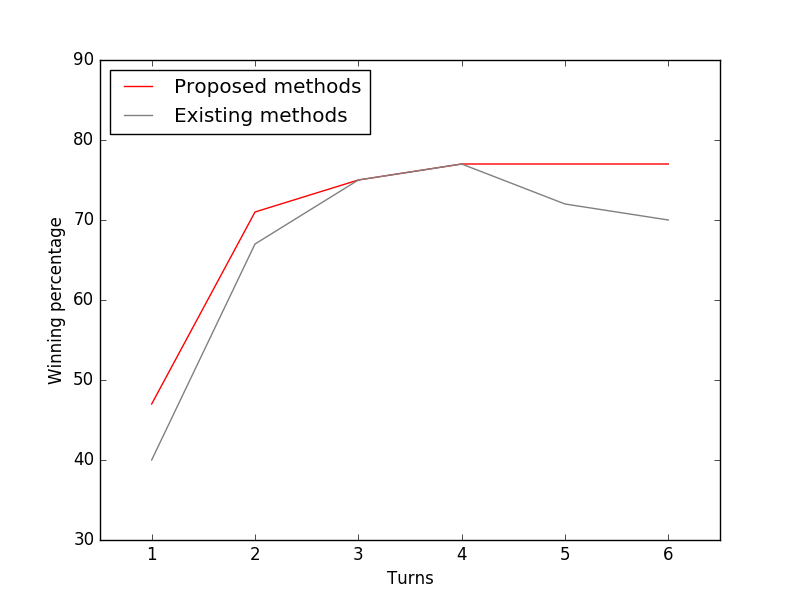
\includegraphics[scale=0.8]{./koki/w.png} \\
   \caption{勝率の比較}
\end{center}
\label{fig:w}
\end{figure}

\begin{figure}[]
\begin{center}
   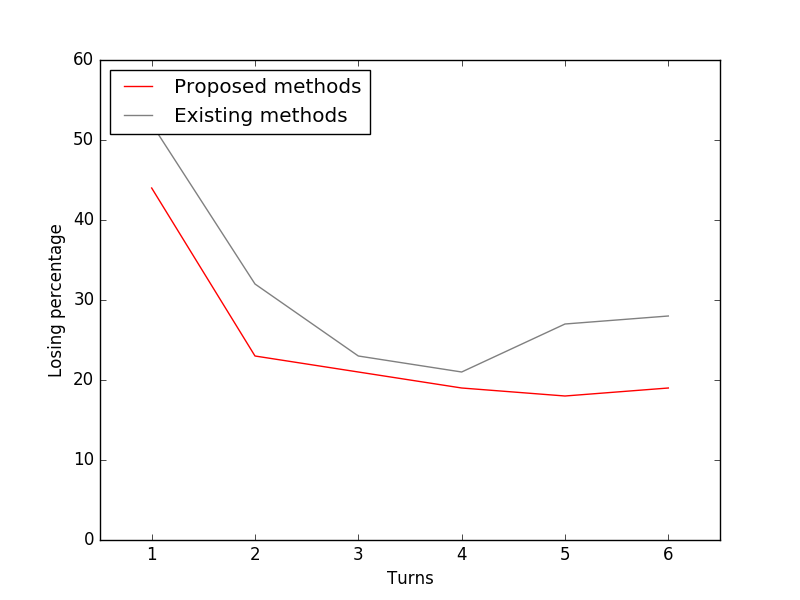
\includegraphics[scale=0.8]{./koki/ll.png} \\
   \caption{敗北率の比較}
\end{center}
\label{fig:ll}
\end{figure}

\begin{figure}[]
\begin{center}
   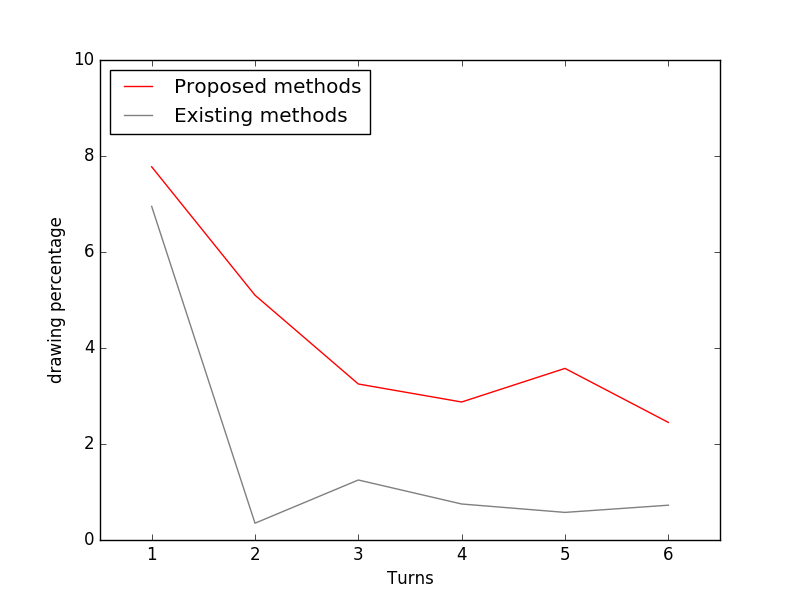
\includegraphics[scale=0.8]{./koki/d.png} \\
   \caption{引き分け率の比較}
\end{center}
\label{fig:d}
\end{figure}

\section{実験結果に対する考察}
図\ref{fig:w}より,提案手法は既存手法に比べ,勝率の点ではほとんど変化が見られず,若干の上昇しか見られなかったものの,図\ref{fig:ll},図\ref{fig:d}より,敗北率の減少と,引き分け率の増加が観察された.

これは,提案手法,既存手法ともに勝利条件に紐づくサブゴールの獲得は共に上手く行っているため,勝率に関しては二手法ともにほとんど変化が見られなかったことが示唆される.
すなわち,現在の盤面が自分に有利な状況,すなわち勝ちにつながりやすい盤面である場合,その盤面の環境を観測してから,勝ち条件をみたすための最適行動を出力する学習は,二手法ともに上手く行っている.

一方,敗北率が減少している点について,提案手法の負のサブゴールの働きにより,上手く敗北濃厚な場面を避けている学習が実現していることがわかる.
既存手法では,敗北を避ける学習を行うことが出来なかった.
三目並べでは,自身が後攻である場合,相手の手によってはどこに打っても勝利盤面へ持っていけない状況が存在する.既存手法では勝利盤面の環境に紐づく盤面しか学習できないため,どこに打っても勝利盤面へ遷移しない状況下において最適行動学習を行うことが出来ない.

一方,提案手法では,敗北時の盤面と紐づく状況も学習することができるため,どこへ打っても勝利に至らない盤面から,敗北を避け,引き分けへと持っていく最適行動が学習できていると考える.


%%!TEX root = ../main.tex
\chapter{結論}
本論文では.IL-RBMを改良し.強化学習タスクへの応用方法を示した.

ニューラルネットワークを用いた強化学習を行うにあたり,ニューラルネットワークにおける有効な追加学習法を考案する必要性があった.

文献\cite{osawa}で提案されたIL-RBMは追加学習が可能であり,与えられたデータが既学習か未学習かを判定することで、自動的に未学習データセットを構築可能であった.またその未学習データセットを用いて追加学習が可能であった.
しかし,IL-RBMはデータの未学習,既学習の判定は可能であるものの,強化学習への応用の際.与えられたデータが正の報酬に関連づくものか.負の報酬に関連づくものかを区別することが出来なかった.

そこで.IL-RBMに正と負の二種類のネットワークを持たせることで.IL-RBMが正の報酬と関連の強いデータと負の報酬と関連の強いデータを区別することが可能であることを示した.

IL-RBMが正のネットワークと負のネットワークを持つことで.既存手法では扱えなかった負のサブゴールを設定可能となり.負の報酬を避けるような長期的な戦略を獲得できることを示した.

また.提案したIL-RBMをもちいたエージェントに三目並べタスクを実際に解かせた.
エージェントは正の報酬へ繋がる行動のデータセットと負の報酬へ繋がる行動のデータセットを採集し.それぞれを提案した正負のネットワークで学習することで.負のネットワークを持たないIL-RBMより高い勝率で勝つことができることを示した.また.負の報酬を避けるような長期的な戦略により.より顕著に敗北率が減少することを示した.

ニューラルネットワークを行う強化学習において、有効な追加学習法を示せたことにより、より抽象度の高い応用例を示すことを今後の課題とする。
\謝辞


%\bibliographystyle{jecon.bst}
\bibliography{./reference/reference}


\appendix

\chapter{評価実験の対話データ}
ここでは、評価実験の際に実際に行われた対話を本編で記した以外のものを記す。

\begin{longtable}{| c | p{15zw} | p{15zw}|}
\caption{20代女性の対話例}
%\label{fig:samplenoboke}
\endhead
%\begin{tabular*}{70mm}{@{\extracolsep{\fill}}|c|c|}\hline %ココ
\hline
{\em 話者} & {\em 発話文} & {\em 応答パターン}\\
\hline
\hline
usr & こんにちは & \\
sys & こんにちは & テンプレート応答\\
usr & 調子はどうですか? & \\
sys & 怒りたい & 攻撃ユーモア(テンプレート応答)\\
usr & どうしてですか? & \\
sys & 他の話をしようぜよ & 応答生成不可or応答候補無し\\
usr & 天気がいいですね & \\
sys & それはいいね! & 極性を考慮した相槌\\
usr & 散歩したいです & \\
sys & え?ランコしたいです?私の聞き間違いですか?? & 遊戯ユーモア(ダジャレ)\\
usr & 聞き間違いです & \\
sys & それは辛いね & 極性を考慮した相槌\\
usr & 辛いです & \\
sys & 君を励ましたかった & 支援ユーモア(テンプレート応答)\\
usr & ありがとう & \\
sys & どういたしまして & テンプレート\\
usr & 元気ですか & \\
sys & さすがです & 相槌\\
\hline
\end{longtable}


\begin{longtable}{| c | p{15zw} | p{15zw}|}
\caption{20代男性の対話例}
%\label{fig:samplenoboke}
\endhead
%\begin{tabular*}{70mm}{@{\extracolsep{\fill}}|c|c|}\hline %ココ
\hline
{\em 話者} & {\em 発話文} & {\em 応答パターン}\\
\hline
\hline
usr & こんにちは & \\
sys & こんにちは & テンプレート応答\\
usr & よろしくおねがいします & \\
sys & うるさいですね & 攻撃ユーモア(テンプレート応答) \\
usr & ごめんなさい & \\
sys & いいえ & テンプレート\\
usr & 最近寒いですね & \\
sys & 他の話をしないか? & 応答生成不可or応答候補無し\\
usr & お金が欲しい & \\
sys & なんて? & 攻撃ユーモア(テンプレート応答)\\
usr & 卒論つらい & \\
sys & なるほどねー。 & 相槌\\
usr & 死にたい & \\
sys & あなたは子孫繁栄が死ねばよかったのに。 & 攻撃ユーモア(ツッコミ)\\
usr & お腹が好きました & \\
sys & 私も好きです & テンプレート応答\\
usr & 僕は嫌いです & \\
sys & なんて?ダツは嫌いです?私の聞き間違いですか?? & 遊戯ユーモア(ダジャレ)\\
usr & あなたの聞き間違いです & \\
sys & あなたを悲しませたい & 攻撃ユーモア(テンプレート応答)\\
usr & やめてください & \\
sys & 他の話をしようぜ? & 応答生成不可or応答候補無し\\
usr & いいよ & \\
sys & 他の話をしようぜ? & 応答生成不可or応答候補無し\\
usr & 音楽が好きです & \\
sys & 私も好きです & テンプレート応答\\
usr & 福神漬が嫌いです & \\
sys & あなたを楽しませたい & 遊戯ユーモア(テンプレート応答)\\
usr & もっと頑張って & \\
sys & 怒りたい & 攻撃ユーモア(テンプレート応答)\\
usr & やめて & \\
sys & え、そうなんだ & 相槌\\
usr & 怒られるのは嫌いだよ & \\
sys & なんて?怒られるのはキレイだよ?私の聞き間違いですか?? & \\
usr & あなたの名前は? & \\
sys & ゼロです。以後お見知りおきを & テンプレート応答\\
usr & よろしくお願いします & \\
sys & こちらこそよろしくお願いします & テンプレート応答\\
usr & かっこいい名前ですね & \\
sys & なんて?かっこいいナナイですね?私の聞き間違いですか?? & \\
usr & かわいい女の子が好き & \\
sys & 私も好きです & テンプレート応答\\
usr & かわいい男の子も好き & \\
sys & 私も好きです & テンプレート応答\\
usr & へえ & \\
sys & 他の話をしようぜ? & 応答生成不可or応答候補無し\\
usr & いいよ & \\
sys & あなたを悲しませたい & 攻撃ユーモア(テンプレート応答)\\
usr & もうやめようよ & \\
sys & 他の話をしようぜよ & 応答生成不可or応答候補無し\\
usr & やめよう & \\
sys & 他の話をしようぜ? & 応答生成不可or応答候補無し\\
usr & 嫌です & \\
sys & あなたを楽しませたい & 遊戯ユーモア(テンプレート応答)\\
usr & 嬉しい & \\
sys & あなたを悲しませたい & 攻撃ユーモア(テンプレート応答)\\
usr & お前きらい & \\
sys & 今から1年経てば、その辛さもどうでも良くなってるよ & \\
usr & いいこと言うね & \\
sys & ごめん、応答が思いつかない & 応答生成不可or応答候補無し\\
usr & もうやめようか & \\
sys & 他の話をしようぜ? & 応答生成不可or応答候補無し\\
usr & ばいばい & \\
sys & へー、ほんとにぃ & 相槌\\
\hline
\end{longtable}



%\chapter{予備実験で得た結果}
ここでは、予備実験で得たユーモアのタイミングや内容を考慮する材料となった表の例を示す。\\
\hspace{1zw}例1はある男性の結果,例2はある女性の結果である。

\begin{table}
\begin{center}
\caption{極性の例1}
\label{tb:ex1PN}
\begin{tabular}{|c|c|c|p{6em}|p{6em}|p{6em}|}
\hline
\multicolumn{1}{|c}{} & \multicolumn{1}{c}{} & \multicolumn{1}{c|}{} & \multicolumn{3}{c|}{全体的にどの極性が多いか} \\
\cline{4-6}
\multicolumn{1}{|c}{} & \multicolumn{1}{c}{} & \multicolumn{1}{c|}{} & \multicolumn{1}{c|}P & \multicolumn{1}{c|}N & \multicolumn{1}{c|}E \\
\hline
 &  & 攻撃ユーモア & \hspace{2.4zw}0.6 & \hspace{2.4zw}0.2 & \hspace{2.4zw}0.2 \\\cline{3-6}
 & P & 支援ユーモア & \hspace{2.4zw}0.3 & \hspace{2.4zw}0.6 & \hspace{2.4zw}0.5 \\\cline{3-6}
 &  & 遊戯ユーモア & \hspace{2.4zw}0.8 & \hspace{2.4zw}0.4 & \hspace{2.4zw}0.3 \\\cline{3-6}
 &  & ユーモア無し & \hspace{2.4zw}0.2 & \hspace{2.4zw}0.2 & \hspace{2.4zw}0.0 \\\cline{2-6}
 &  & 攻撃ユーモア & \hspace{2.4zw}0.6 & \hspace{2.4zw}0.7 & \hspace{2.4zw}0.0 \\\cline{3-6}
1つ前の & N & 支援ユーモア & \hspace{2.4zw}0.7 & \hspace{2.4zw}0.7 & \hspace{2.4zw}0.5 \\\cline{3-6}
ユーザの &  & 遊戯ユーモア & \hspace{2.4zw}0.5 & \hspace{2.4zw}0.5 & \hspace{2.4zw}0.5 \\\cline{3-6}
発話極性 &  & ユーモア無し & \hspace{2.4zw}0.2 & \hspace{2.4zw}0.2 & \hspace{2.4zw}0.0 \\\cline{2-6}
 &  & 攻撃ユーモア & \hspace{2.4zw}0.6 & \hspace{2.4zw}0.6 & \hspace{2.4zw}0.6 \\\cline{3-6}
 & E & 支援ユーモア & \hspace{2.4zw}0.3 & \hspace{2.4zw}0.4 & \hspace{2.4zw}0.3 \\\cline{3-6}
 &  & 遊戯ユーモア & \hspace{2.4zw}0.7 & \hspace{2.4zw}0.8 & \hspace{2.4zw}0.7 \\\cline{3-6}
 &  & ユーモア無し & \hspace{2.4zw}0.1 & \hspace{2.4zw}0.2 & \hspace{2.4zw}0.2 \\\hline
\end{tabular}
\end{center}
\end{table}


\begin{table}
\begin{center}
\caption{態度の例1}
\label{tb:ex1taido}
\begin{tabular}{|c|c|c|p{6em}|p{6em}|}
\hline
\multicolumn{1}{|c}{} & \multicolumn{1}{c}{} & \multicolumn{1}{c|}{} & \multicolumn{2}{c|}{全体的に態度が良いか否か} \\\cline{4-5}
\multicolumn{1}{|c}{} & \multicolumn{1}{c}{} & \multicolumn{1}{c|}{} & \hspace{2zw}多い & \hspace{1.5zw}少ない \\\hline
 &  & 攻撃ユーモア & \hspace{2.4zw}0.4 & \hspace{2.4zw}0.6 \\\cline{3-5}
 & 良い & 支援ユーモア & \hspace{2.4zw}0.5 & \hspace{2.4zw}0.5 \\\cline{3-5}
 &  & 遊戯ユーモア & \hspace{2.4zw}0.3 & \hspace{2.4zw}0.6 \\\cline{3-5}
 今のユーザの &  & ユーモア無し & \hspace{2.4zw}0.2 & \hspace{2.4zw}0.3 \\\cline{2-5}
態度が &  & 攻撃ユーモア & \hspace{2.4zw}0.5 & \hspace{2.4zw}0.7 \\\cline{3-5}
良いか否か & 悪い & 支援ユーモア & \hspace{2.4zw}0.4 & \hspace{2.4zw}0.3 \\\cline{3-5}
 &  & 遊戯ユーモア & \hspace{2.4zw}0.4 & \hspace{2.4zw}0.5 \\\cline{3-5}
 &  & 無し & \hspace{2.4zw}0.3 & \hspace{2.4zw}0.4 \\\hline
\end{tabular}
\end{center}
\end{table}

\begin{table}[tb]
\begin{center}
\caption{ユーモアの連続性の例1}
\label{tb:ex1humor}
\begin{tabular}{| c | c |}
\hline
     \multicolumn{2}{| c |}{ユーモアの連続性} \\\hline
     攻撃ユーモアの連続性 & 0.3 \\\hline
     支援ユーモアの連続性 & 0.5 \\\hline
	 遊戯ユーモアの連続性 & 0.6 \\\hline
     
\end{tabular}
\end{center}
\end{table}




\begin{table}[tb]
\begin{center}
\caption{重みづけの例1}
\label{tb:ex1weight1}
\begin{tabular}{| c | c |}
\hline
     \multicolumn{2}{| c |}{重みづけ} \\\hline
	 ユーザの態度 & 0.1 \\\hline
     入力文の極性 & 0.5 \\\hline
	 ユーモアの連続性 & 0.4 \\\hline
     
\end{tabular}
\end{center}
\end{table}



\begin{table}
\begin{center}
\caption{極性の例2}
\label{tb:ex1PN}
\begin{tabular}{|c|c|c|p{6em}|p{6em}|p{6em}|}
\hline
\multicolumn{1}{|c}{} & \multicolumn{1}{c}{} & \multicolumn{1}{c|}{} & \multicolumn{3}{c|}{全体的にどの極性が多いか} \\
\cline{4-6}
\multicolumn{1}{|c}{} & \multicolumn{1}{c}{} & \multicolumn{1}{c|}{} & \multicolumn{1}{c|}P & \multicolumn{1}{c|}N & \multicolumn{1}{c|}E \\
\hline
 &  & 攻撃ユーモア & \hspace{2.4zw}0.8 & \hspace{2.4zw}0.2 & \hspace{2.4zw}0.3 \\\cline{3-6}
 & P & 支援ユーモア & \hspace{2.4zw}0.4 & \hspace{2.4zw}0.8 & \hspace{2.4zw}0.5 \\\cline{3-6}
 &  & 遊戯ユーモア & \hspace{2.4zw}0.7 & \hspace{2.4zw}0.5 & \hspace{2.4zw}0.6 \\\cline{3-6}
 &  & ユーモア無し & \hspace{2.4zw}0.4 & \hspace{2.4zw}0.6 & \hspace{2.4zw}0.5 \\\cline{2-6}
 &  & 攻撃ユーモア & \hspace{2.4zw}0.6 & \hspace{2.4zw}0.6 & \hspace{2.4zw}0.5 \\\cline{3-6}
1つ前の & N & 支援ユーモア & \hspace{2.4zw}0.7 & \hspace{2.4zw}0.8 & \hspace{2.4zw}0.6 \\\cline{3-6}
ユーザの&  & 遊戯ユーモア & \hspace{2.4zw}0.5 & \hspace{2.4zw}0.6 & \hspace{2.4zw}0.5 \\\cline{3-6}
発話極性 &  & ユーモア無し & \hspace{2.4zw}0.5 & \hspace{2.4zw}0.3 & \hspace{2.4zw}0.4 \\\cline{2-6}
 &  & 攻撃ユーモア & \hspace{2.4zw}0.7 & \hspace{2.4zw}0.5 & \hspace{2.4zw}0.6 \\\cline{3-6}
 & E & 支援ユーモア & \hspace{2.4zw}0.7 & \hspace{2.4zw}0.8 & \hspace{2.4zw}0.6 \\\cline{3-6}
 &  & 遊戯ユーモア & \hspace{2.4zw}0.5 & \hspace{2.4zw}0.5 & \hspace{2.4zw}0.4 \\\cline{3-6}
 &  & ユーモア無し & \hspace{2.4zw}0.5 & \hspace{2.4zw}0.4 & \hspace{2.4zw}0.6 \\\hline
\end{tabular}
\end{center}
\end{table}


\begin{table}
\begin{center}
\caption{態度の例2}
\label{tb:ex1taido}
\begin{tabular}{|c|c|c|p{6em}|p{6em}|}
\hline
\multicolumn{1}{|c}{} & \multicolumn{1}{c}{} & \multicolumn{1}{c|}{} & \multicolumn{2}{c|}{全体的に態度が良いか否か} \\\cline{4-5}
\multicolumn{1}{|c}{} & \multicolumn{1}{c}{} & \multicolumn{1}{c|}{} & \hspace{2zw}多い &\hspace{1.5zw}少ない \\\hline
 &  & 攻撃ユーモア & \hspace{2.4zw}0.2 & \hspace{2.4zw}0.3 \\\cline{3-5}
 & 良い & 支援ユーモア & \hspace{2.4zw}0.7 & \hspace{2.4zw}0.2 \\\cline{3-5}
 &  & 遊戯ユーモア & \hspace{2.4zw}0.3 & \hspace{2.4zw}0.1 \\\cline{3-5}
 今のユーザの &  & ユーモア無し & \hspace{2.4zw}0.4 & \hspace{2.4zw}0.3 \\\cline{2-5}
態度が &  & 攻撃ユーモア & \hspace{2.4zw}0.3 & \hspace{2.4zw}0.4 \\\cline{3-5}
良いか否か & 悪い & 支援ユーモア & \hspace{2.4zw}0.6 & \hspace{2.4zw}0.3 \\\cline{3-5}
 &  & 遊戯ユーモア & \hspace{2.4zw}0.4 & \hspace{2.4zw}0.2 \\\cline{3-5}
 &  & 無し & \hspace{2.4zw}0.5 & \hspace{2.4zw}0.6 \\\hline
\end{tabular}
\end{center}
\end{table}

\begin{table}[tb]
\begin{center}
\caption{ユーモアの連続性の例2}
\label{tb:ex1humor}
\begin{tabular}{| c | c |}
\hline
     \multicolumn{2}{| c |}{ユーモアの連続性} \\\hline
     攻撃ユーモアの連続性 & 0.2 \\\hline
     支援ユーモアの連続性 & 0.6 \\\hline
	 遊戯ユーモアの連続性 & 0.5 \\\hline
     
\end{tabular}
\end{center}
\end{table}




\begin{table}[tb]
\begin{center}
\caption{重みづけの例2}
\label{tb:ex1weight1}
\begin{tabular}{| c | c |}
\hline
     \multicolumn{2}{| c |}{重みづけ} \\\hline
	 ユーザの態度 & 0.5 \\\hline
     入力文の極性 & 0.3 \\\hline
	 ユーモアの連続性 & 0.2 \\\hline
     
\end{tabular}
\end{center}
\end{table}


\end{document}